
\chapter{量子随机行走搜索算法的实验实现}



量子随机行走(quantum random walk),又称量子游走或者很文艺的量子漫步,是经典随机行走的量子版本。正是由于经典行走在设计随机算法
中的广泛应用及较低效率,2001年Ambainis, Kempe和Childs等人提出可以利用量子随机行走开发量子算法,拟对这些问题提供量子加速性\cite{rwview1,rwview2,rwview3}。对一些经典上的
难问题,例如黑盒子问题,量子随机行走可以提供指数加速\cite{rwview4,rwview5},而对于另外一些特定问题,比如
元素分离问题\cite{rwview6},三角搜索问题\cite{rwview7},NAND树判断问题\cite{rwview8}等等,可以提供多项式加速。

在本章中,我们主要关注的是基于量子随机行走过程的搜索算法(SKW算法)\cite{skw},以及其在NMR上的首次实验实现\cite{rw1}。在第一节中,我们会从
经典随机行走出发,介绍量子随机行走的两种形式:离散的和连续的;然后我们会介绍SKW算法的理论实现过程,并给出该算法与
著名的Grover搜索算法\cite{grover}之间的比较;在本章的最后,我们会从NMR实验的角度介绍SKW算法的首次实现,并作相应的讨论及展望。

\section{量子随机行走的简介}

“\emph{上帝是不掷骰子的。}”

 \hspace{19em} \emph{--阿尔伯特·爱因斯坦}

\subsection{经典随机行走}

经典随机行走起源于1905年爱因斯坦发表的关于布朗运动的研究论文\cite{crw}。在那之后一个世纪,关于布朗运动以及相关的随机行走模型的研究
有了长足的进展,不仅在物理学中,也在其他的学科比如化学,地理,生物甚至经济学中都被广泛应用。作为马尔科夫过程,随机行走可以在任意的图上实现。让我们来看一个关于经典随机行走的简单的例子。

不失一般性,我们考虑一个一维晶格上的随机行走过程。假设一维晶格上一共存在$N$个格点,每个格点都用一个正整数或者负整数来标记,如图\ref{crw}(a)所示,所有的格点从-9到+9依次标记。在每一次行走后,我们都只能处在
某个格点上,同时假设我们初始时呆在0处。然后我们抛掷一枚经典的硬币,它只能朝上或者朝下。当硬币朝上时,我们往左走一步,反之则往右走一步。在一定的步数$T$之后,
我们可以计算行走者处在每个格点上的概率(图\ref{crw}(b))。当然,我们也可以选择两个方向是不等概率的,即硬币处于朝上和朝下的概率是不同的。

\begin{figure}[htbp]
            \begin{center}
              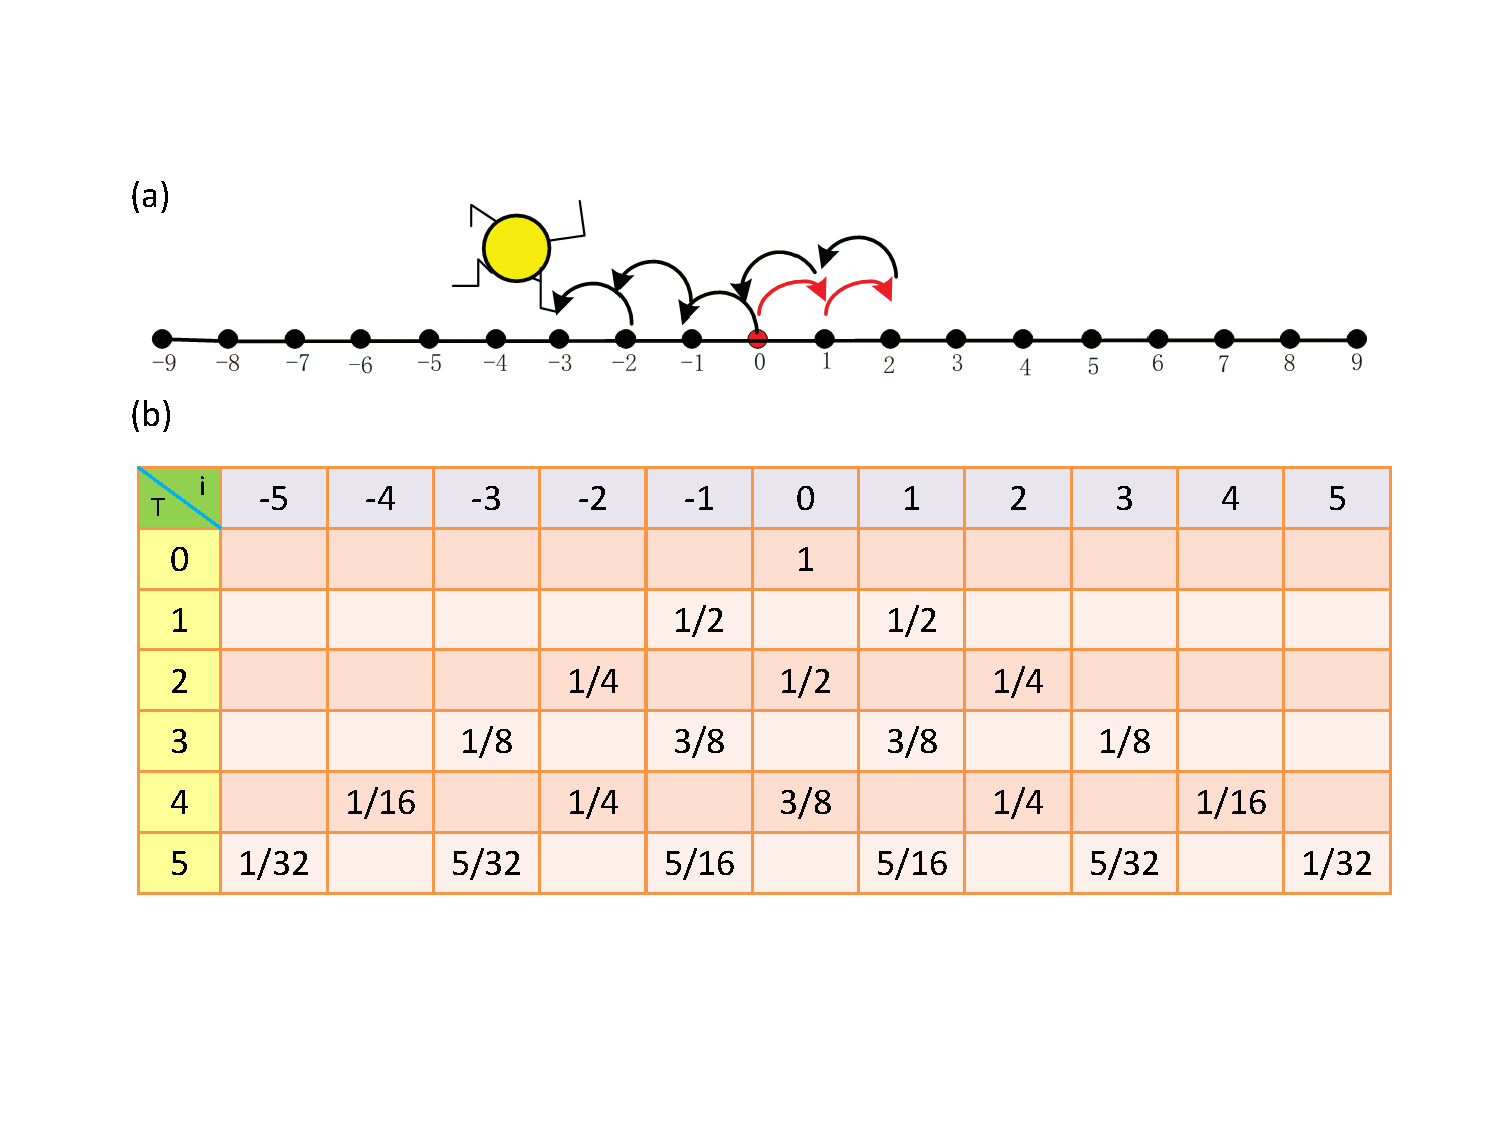
\includegraphics[width= 0.8\columnwidth]{figures/crw.pdf}
              \caption{(a) 一维晶格上,行走者可以通过投掷硬币来决定两个行走的方向。取自[Theoretical Computer Science 394, 817 (2008)]\cite{crw2}。(b) 一维晶格上经过$T$次行走之后行走者所处的状态。可以看出,行走者处于中间的位置大于处于两端的概率。
              }
              \label{crw}
            \end{center}
        \end{figure}

依据概率论的知识,在经过足够长的步数之后,行走者所处位置的概率分布为
\begin{equation}
          \rho(x,T) = \frac{1}{\sqrt{2\pi T}}e^{-\frac{x^2}{2T}},
 \end{equation}
 其中$x$表示一维晶格上的位置。可以看出,行走者所处位置的概率分布为Gauss分布,最终所处的位置平均值为0, 且位置的协方差为 $\sigma^2 = T$。因此从统计的角度看行走者距离中心的距离是和步数的平方根成正比的。

 \subsection{离散型量子随机行走}

 在经典行走过程中,行走者每次只能朝一个方向走。而在量子化的行走过程中,由于量子力学的叠加性,量子行走者可以朝两边同时走,除非被测量塌缩
 (图\ref{qrw})。而在量子随机行走中,目前主要分为两种:离散型(discrete time)与连续型(continuous time)。本节我们介绍离散型量子随机行走。

 \begin{figure}[htbp]
            \begin{center}
              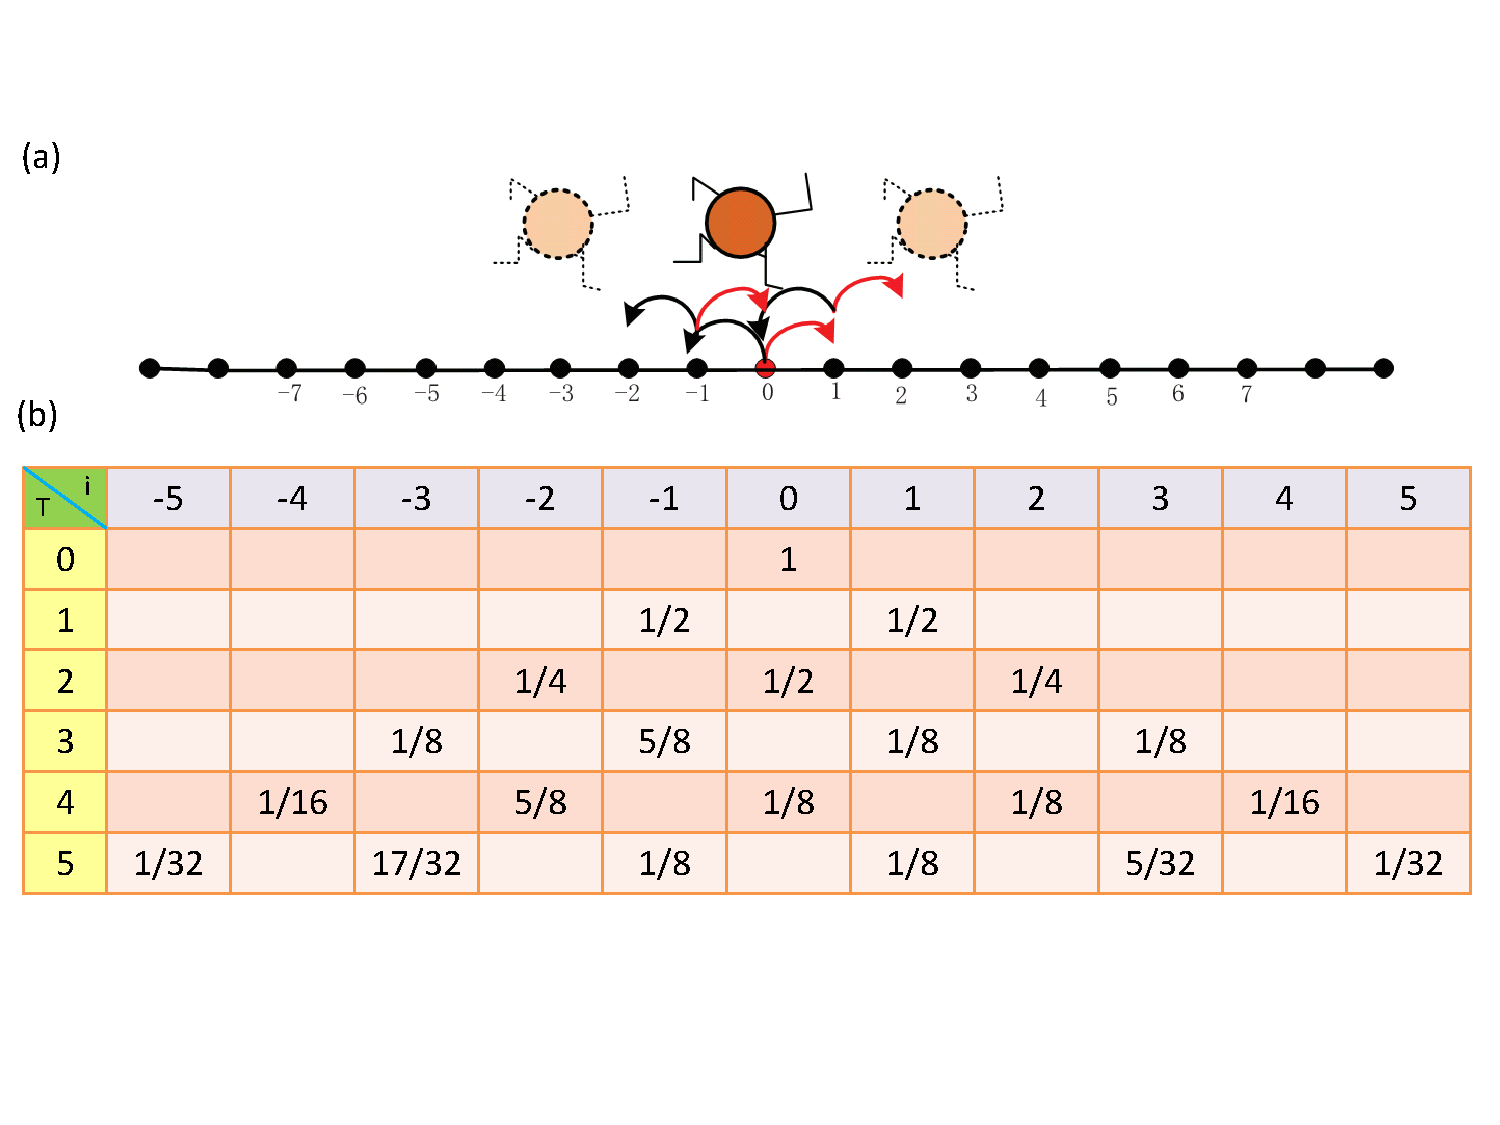
\includegraphics[width= 0.8\columnwidth]{figures/qrw.pdf}
              \caption{(a)量子行走的原理性示意图。行走者可以通过量子硬币的状态同时朝左和朝右行走,正体现了量子力学的奇异性质。取自[Theoretical Computer Science 394, 817 (2008)]\cite{crw2}。(b)离散型量子随机行走的情况在$T$步之后的概率分布。系统初态为$\left\vert \Phi_{in} \right \rangle = \left\vert \downarrow \right \rangle \otimes \left\vert 0 \right \rangle$。注意到从$T=3$开始量子行走与经典行走的差异就显现出来了。
              }
              \label{qrw}
            \end{center}
 \end{figure}

 离散型量子随机行走又叫硬币型量子随机行走(coin quantum random walk)。顾名思义,在离散型中,我们需要一枚量子硬币。简单起见,我们依然只讨论一维晶格上的离散型量子随机行走。

 在离散型中,我们要定义两个Hilbert空间
\begin{equation}
          H = H_c\otimes H_p,
\end{equation}
 其中$H_c$是硬币的Hilbert空间而$H_p$是位置空间,有如下形式
\begin{equation}
          H_p = \{\left\vert x \right \rangle; x\in \mathcal{Z} \}, H_c = \{\left\vert \uparrow \right \rangle, \left\vert \downarrow \right \rangle\},
\end{equation}
$x$代表位置。在硬币空间中,$\left\vert \uparrow \right \rangle$指向右走,而$\left\vert \downarrow \right \rangle$指向左走。在离散型量子随机行走中,行走算符为以下形式
 \begin{equation}
          S =\left\vert \uparrow \right \rangle \left\langle \uparrow \right \vert \otimes \sum_x \left\vert x+1 \right \rangle  \left\langle x \right \vert +\left\vert \downarrow \right \rangle \left\langle \downarrow \right \vert \otimes \sum_x \left\vert x-1 \right \rangle  \left\langle x \right \vert,
\end{equation}
其作用是把态$\left\vert\uparrow \right \rangle \otimes  \left\vert x \right \rangle $转化为 $\left\vert \uparrow \right \rangle \otimes  \left\vert x+1 \right \rangle $,而把$\left\vert \downarrow \right \rangle \otimes  \left\vert x \right \rangle $转化为$\left\vert \downarrow \right \rangle \otimes  \left\vert x-1 \right \rangle $。

量子随机行走的第一步依然是对硬币的抛掷,类似于经典随机行走,我们一般称之为抛硬币(coin flip)算符$C$。对于$C$的选取是任意的,而由此表现出的量子随机行走的性质也是多种多样的。常用的抛硬币方法为Hadamard操作
\begin{equation}
          C = \frac{1}{\sqrt{2}}\left(
                \begin{array}{cc}
                  1 & 1 \\
                  1& -1 \\
                \end{array}
              \right),
\end{equation}
这是一个"平衡"的量子硬币。假设行走者初始处于$\left\vert 0 \right \rangle$,而硬币处于$\left\vert\uparrow \right \rangle$的话,经过一次抛硬币及行走后,系统的状态将变为
\begin{equation}
          \left\vert \uparrow \right \rangle \otimes\left\vert 0 \right \rangle \underrightarrow{C}  \frac{1}{\sqrt{2}}(\left\vert \uparrow \right \rangle +\left\vert \downarrow \right \rangle) \otimes\left\vert 0 \right \rangle
          \underrightarrow{S} \frac{1}{\sqrt{2}}(\left\vert \uparrow \right \rangle \otimes  \left\vert 1 \right \rangle + \left\vert \downarrow \right \rangle \otimes \left\vert -1 \right \rangle).
\end{equation}
这时如果对硬币状态在计算基矢中的测量将给出$\{\left\vert \uparrow \right \rangle \otimes  \left\vert 1 \right \rangle,  \left\vert \downarrow \right \rangle \otimes \left\vert -1 \right \rangle\}$的概率均为1/2。如果我们每次行走后都进行测量的话,那么这就蜕化到了经典随机行走的形式。

在量子随机行走中,我们当然不会每走完一步就进行塌缩测量,也就是每一步之后我们都保持了不同位置间的量子关联,并让它们在
接下来的行走中继续互相干涉。正是这种干涉导致了量子行走的奇异行为。

定义量子行走了$T$步的幺正算子为$U^T$,显然$U$的形式为
 \begin{equation}
          U = S\cdot(C\otimes I).
\end{equation}
假设我们的初态为$\left\vert \Phi_{in} \right \rangle = \left\vert \downarrow \right \rangle \otimes \left\vert 0 \right \rangle$,那么考虑行走几步后的情况(当然保证中间不进行任何测量)
\begin{eqnarray}
   \left\vert \Phi_{in} \right \rangle  & \underrightarrow{U}   &  \frac{1}{\sqrt{2}}(\left\vert \uparrow \right \rangle \otimes  \left\vert 1 \right \rangle - \left\vert \downarrow \right \rangle \otimes \left\vert -1 \right \rangle) \nonumber \\
   & \underrightarrow{U}   &  \frac{1}{\sqrt{2}}(\left\vert \uparrow \right \rangle \otimes  \left\vert 2 \right \rangle -
  (\left\vert \uparrow \right \rangle-\left\vert \downarrow \right \rangle) \otimes  \left\vert 0 \right \rangle+
  \left\vert \downarrow \right \rangle \otimes \left\vert -2 \right \rangle) \nonumber \\
   & \underrightarrow{U}   & \frac{1}{\sqrt{2\sqrt{2}}}(\left\vert \uparrow \right \rangle \otimes  \left\vert 3 \right \rangle + \left\vert \downarrow \right \rangle \otimes  \left\vert 1 \right \rangle+\left\vert \uparrow \right \rangle \otimes  \left\vert -1 \right \rangle-2\left\vert \downarrow \right \rangle \otimes  \left\vert -1 \right \rangle-\left\vert \downarrow \right \rangle \otimes  \left\vert -3 \right \rangle).
\end{eqnarray}
我们已经发现得到的结果和经典不同了,经典行走的结果(图\ref{crw}(b))与量子行走的结果(图\ref{qrw}(b))对比一目了然。

在这个模型中,值得注意的有两点。其一,明显地,最后得到的概率分布是不对称的,而是"左重右轻"的形式。我们行走100步后,这种非对称性更加明显,见图\ref{rwsym}(a)。这种非对称性起源于Hadamard硬币对于两个方向
$\left\vert\uparrow \right \rangle$和$\left\vert \downarrow \right \rangle$的处理是不同的,它会在$\left\vert \downarrow \right \rangle$前面产生一个-1的相位。直观来看,这个相位会消除掉很多往右走的步数,而使行走者集中于往左走。如果我们把系统的初始状态定为
$\left\vert \Phi_{in} \right \rangle = \left\vert \uparrow \right \rangle \otimes \left\vert 0 \right \rangle$的话我们会发现对称性又变为"右重左轻"。我们可以通过选择对称的输入态
$\left\vert \Phi_{sym} \right \rangle = \frac{1}{\sqrt{2}}(\left\vert \uparrow \right \rangle+ i\left\vert\downarrow \right \rangle)\otimes \left\vert 0 \right \rangle$,或者把抛硬币操作定义为
\begin{equation}
          C = \frac{1}{\sqrt{2}}\left(
                \begin{array}{cc}
                  1 & i \\
                  i& 1 \\
                \end{array}
              \right)
\end{equation}
来消除这种非对称性,见图\ref{rwsym}(b)。

\begin{figure}[htbp]
            \begin{center}
              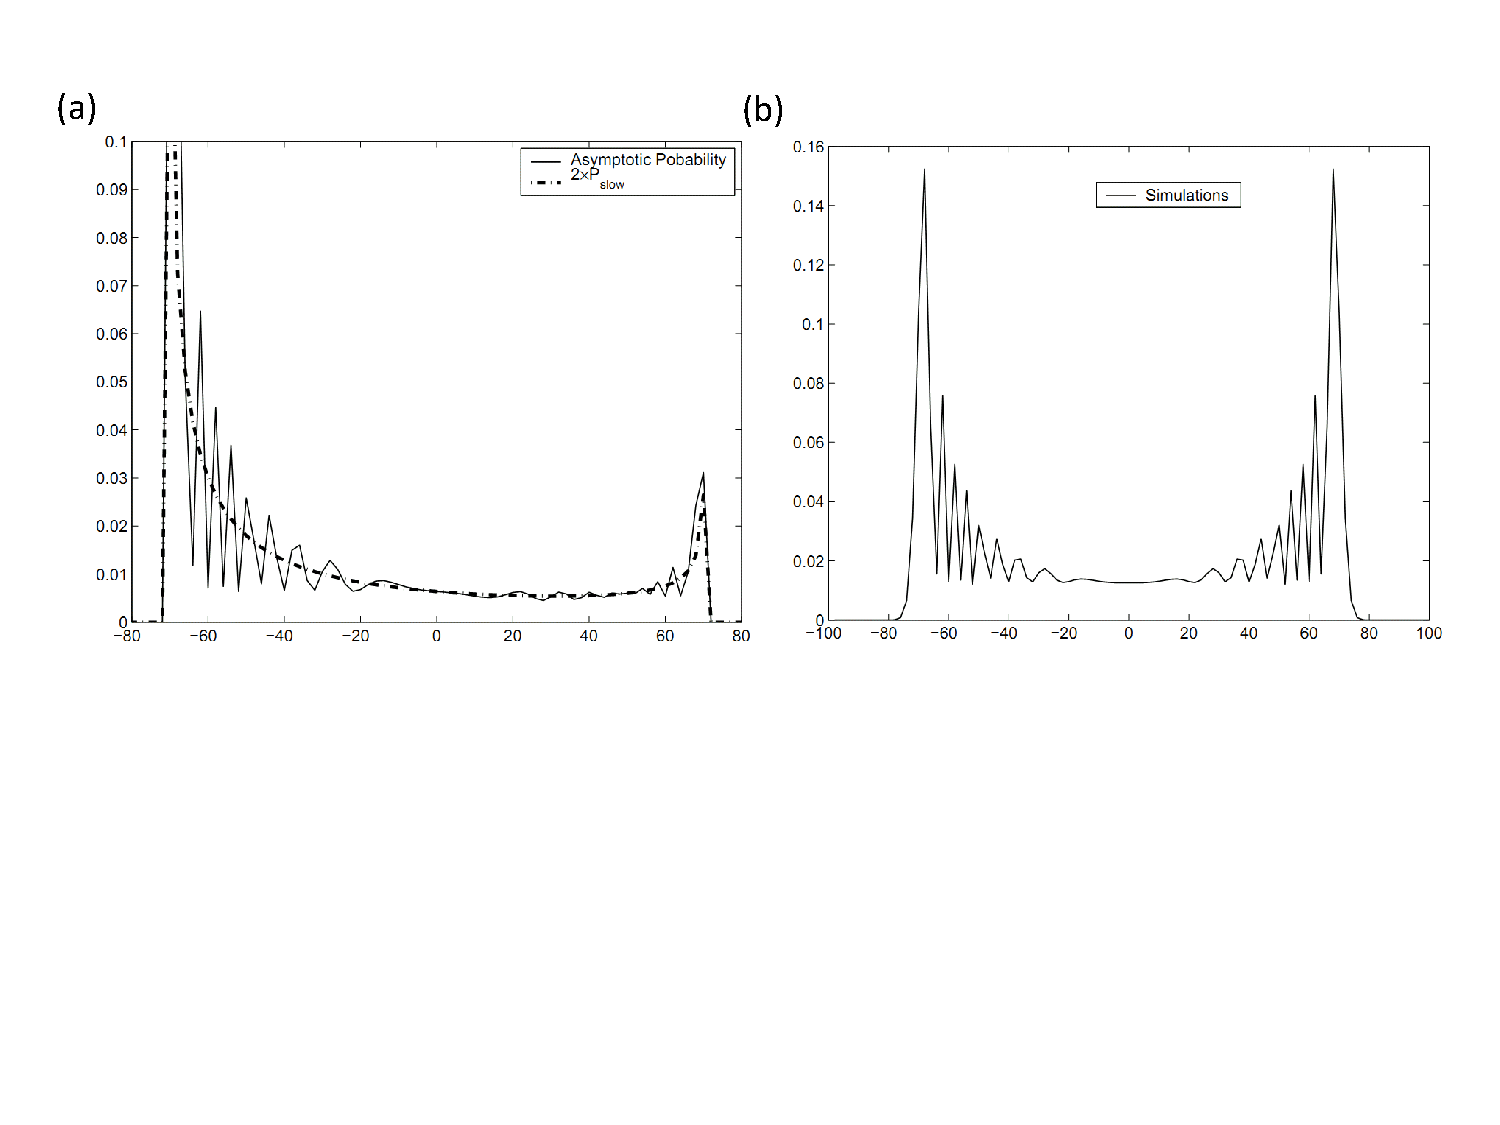
\includegraphics[width= 0.8\columnwidth]{figures/rwsym.pdf}
              \caption{(a)初态为$\left\vert \Phi_{in} \right \rangle = \left\vert \downarrow \right \rangle \otimes \left\vert 0 \right \rangle$的系统在经历100步行走后的概率分布,使用的为Hadamard硬币。可以看出概率分布是"左重右轻"的。(b)如果输入态的形式是对称的,在100步行走之后概率分布依然是对称的。这里只取了处于偶数位置的概率,因为奇数的位置上概率都为0。
              取自[Contemp. Phys. 44, 307 (2003)]\cite{rwview2}。
              }
              \label{rwsym}
            \end{center}
 \end{figure}

另外值得注意的是量子随机行走的概率分布是很复杂的,而且和直觉不同,越往两边概率越大。这正是量子世界的奇异性质的体现。这种分布是很难精确分析的,
Ambainis等人利用费曼路径积分理论给出了一个渐进分析\cite{crw3}。

在经典随机行走中,$T$步之后系统的协方差为$\sigma^2 = T$,也就是距离初始点的期望距离为$\sigma = \sqrt{T}$。而在量子随机行走中,协方差的值为$\sigma^2 \propto T^2$,也就是距离初始点的期望距离为
$\sigma \propto T$,这表明量子随机行走是有二次加速的。

\subsection{连续型量子随机行走}

连续型量子随机行走的模型是由Farhi等人在1998年提出的\cite{crw4}。连续型初看上去与离散型量子随机行走大相径庭,但它们还是有很多相似性的。

在连续型中,我们并不需要硬币空间,也不需要抛硬币。全部的行走过程都发生在位置空间$H_P$中。连续型量子随机行走的
思路来源于经典的连续型马尔科夫过程,所以经常借助于图来进行描述。定义经典上顶点集合为$V$的图,经典行走的一步可以用一个矩阵来描述,该矩阵会使$V$上的概率分布
进行转换。假设$M_{i,j}$给出一次行走中从$i$到$j$的概率,并定义
 \begin{equation}
          \overrightarrow{p}^t = (p_1^t,p_2^t, \cdots , p_{|V|}^t )
\end{equation}
为时间$t$时的概率分布,则有
 \begin{equation}\label{conti}
          p_i^{t+1} = \sum_jM_{i,j}p_j^t,
\end{equation}
也就意味着
\begin{equation}
         \overrightarrow{p}^{t+1} = M \overrightarrow{p}^t.
\end{equation}
$M_{i,j}$是从$i$到$j$的概率,那么最简单的情况是该概率为$1/d_{i}$,$d_i$为$i$的维度。在这种情况下,初始态
\begin{equation}
         \overrightarrow{p}^{0} = (1,0,\ldots,0)
\end{equation}
将行走到
\begin{equation}
         \overrightarrow{p}^{1} = (0,1/2,\ldots,0,1/2),
\end{equation}
继而
\begin{eqnarray}
         \overrightarrow{p}^{2} = (1/2,0,1/4,0,\ldots,0,1/4,0), \nonumber \\
         \overrightarrow{p}^{3} = (0, 3/8,0,1/8,0,\ldots,0,1/8,0,3/8)
\end{eqnarray}
等等,以此类推。

为了使这个过程连续化,我们可以假定所有的行走都是一直发生的,而从一个顶点跳到它邻接顶点的概率为$\gamma$。描述这一过程的矩阵为
\begin{equation}
         H_{i,j} =\left\{
                    \begin{array}{ll}
                      -\gamma, & \hbox{i$\neq$ j 且邻接;} \\
                      0, & \hbox{i$\neq$ j 且不邻接;} \\
                      d_i \gamma, & \hbox{i =j.}
                    \end{array}
                  \right.
\end{equation}
在这种形式下,式\ref{conti}将用完全不同的方程描述
\begin{equation}
         \frac{dp_i(t)}{dt} = -\sum_j H_{i,j}p_j(t).
\end{equation}
求解这个方程将给出
\begin{equation}
         \overrightarrow{p}(t) = e^(-Ht)\overrightarrow{p}(0).
\end{equation}

我们只要把上面的部分转化到其量子版本就是连续型量子随机行走了。描述行走过程的矩阵被哈密顿量替代,
那么行走的算子将变为
\begin{equation}
         U(t)=e^{-iHt}.
\end{equation}
如果我们从某个初态$\left\vert \Phi_{in} \right \rangle$出发,在幺正算子$U$下演化一段时间$T$,并对末态的位置进行测量后,也可以得到类似上面的图上顶点的
概率分布。这就是连续型量子随机行走的概念。更多详细的讲解请参见文献\cite{rwview2}。

\section{SKW算法}

量子随机行走最早都是应用在图上,并且体现出了很多经典行走没有的性质。第一个把量子随机行走应用在算法上,并得到
超越经典算法的速度的方案则是Shenvi, Kempe和Whaley提出的基于量子随机行走的搜索算法\cite{skw}。该算法表明在数据库为$N$的黑箱搜索问题中,我们只需要$O(\sqrt{N})$次
黑箱操作,就可以得到和Grover搜索算法类似的加速效果。本节我们将回顾SKW算法,并把它和著名的Grover搜索算法\cite{grover}作一个比较。

\subsection{SKW算法过程}

我们把搜索空间定义为$n$比特所有的二维向量组$\overrightarrow{x} = \{0,1\}^n$。考虑函数$f(\overrightarrow{x}) = \{0,1\}$,仅仅对一个输入态$\overrightarrow{x} _{target}$时$f(\overrightarrow{x}) =1$ ,而我们的目的就是找到这个$\overrightarrow{x} _{target}$。将$n$比特的二维向量组映射为超立方体上的节点的话,该搜索问题就与在$n$维立方体的$N =2^n$个顶点上搜索一个标记的节点等价。不失一般性,我们可以假设要搜索的节点为 $\overrightarrow{x} _{target} = \overrightarrow{0}$。

SKW算法的过程可以如下描述:

(1) 把量子系统制备到所有的态的等权重叠加上,$\left\vert \psi_{0} \right \rangle = \left\vert s^C \right \rangle \otimes \left\vert s^S \right \rangle $。这一步可以在节点空间的$\overrightarrow{0}$态上施加$n$个单比特Hadamard操作来轻松实现。

(2) 定义一个硬币的黑箱操作$C'$,对于非标记的态,$C_0 = G$,而对于标记的态,$C_1 = -\Gamma$。把整个幺正算子$U' = SC'$作用$t_f = \pi/2\sqrt{2^n}$次。

(3) 在$\left\vert d,\overrightarrow{x} \right \rangle$基矢下测量系统的末态。

SKW证明,最终测量后的输出结果将有$1/2-O(1/n)$的概率得到被标记的态。如果我们把该算法重复大量次的话,
被标记的态就可以以很高的精度确定。其证明过程比较复杂,这里就只给出大致的思路,具体的过程可以参见文献\cite{skw}。

由于需要确定的是$(U')^t$作用在初态$\left\vert \psi_{0} \right \rangle$上的结果,首先SKW把这个问题从在超立方体上的行走塌缩为一维线上的行走。然后,通过近似地构造$U'$的两个本征态
$\left\vert \psi_{0} \right \rangle$和$\left\vert \psi_{1} \right \rangle$,SKW证明$U'$中只有精确的两个本征值是相关的,即初态$\left\vert \psi_{0} \right \rangle$和相关的本征态张成的空间有很高的交叠度。这两个本征值被写成$e^{i\omega_0'}$与$e^{-i\omega_0'}$,而其相关的本征态
$\left\vert \omega_0' \right \rangle$与$\left\vert -\omega_0' \right \rangle$可以写为初态$\left\vert \psi_{0} \right \rangle$和第二个态$\left\vert \psi_{1} \right \rangle$之间的线性组合。这样做后,整个搜索问题就近似转化为在$\left\vert \omega_0' \right \rangle$与$\left\vert -\omega_0' \right \rangle$平面上的二维旋转,从初态
\begin{equation}
     \left\vert \psi_{0} \right \rangle \approx 1/\sqrt{2}(\left\vert \omega_0' \right \rangle+\left\vert -\omega_0' \right \rangle)
\end{equation}
演化到末态
\begin{equation}
     \left\vert \psi_{1} \right \rangle \approx 1/\sqrt{2}(-\left\vert \omega_0' \right \rangle+\left\vert -\omega_0' \right \rangle).
\end{equation}
末态的形式已经和目标态$\left\vert \overrightarrow{x} _{target} \right \rangle $非常接近。最后,SKW证明每执行一次幺正算子$U'$,旋转角度的大小约为$1/\sqrt{2^{n-1}}$。因此,在行走大概$(\pi/2)\sqrt{2^{n-1}}$步后,也就是$O(\sqrt{N})$次黑箱操作后,整个
搜索过程就可以完成了。


\begin{figure}[htbp]
            \begin{center}
              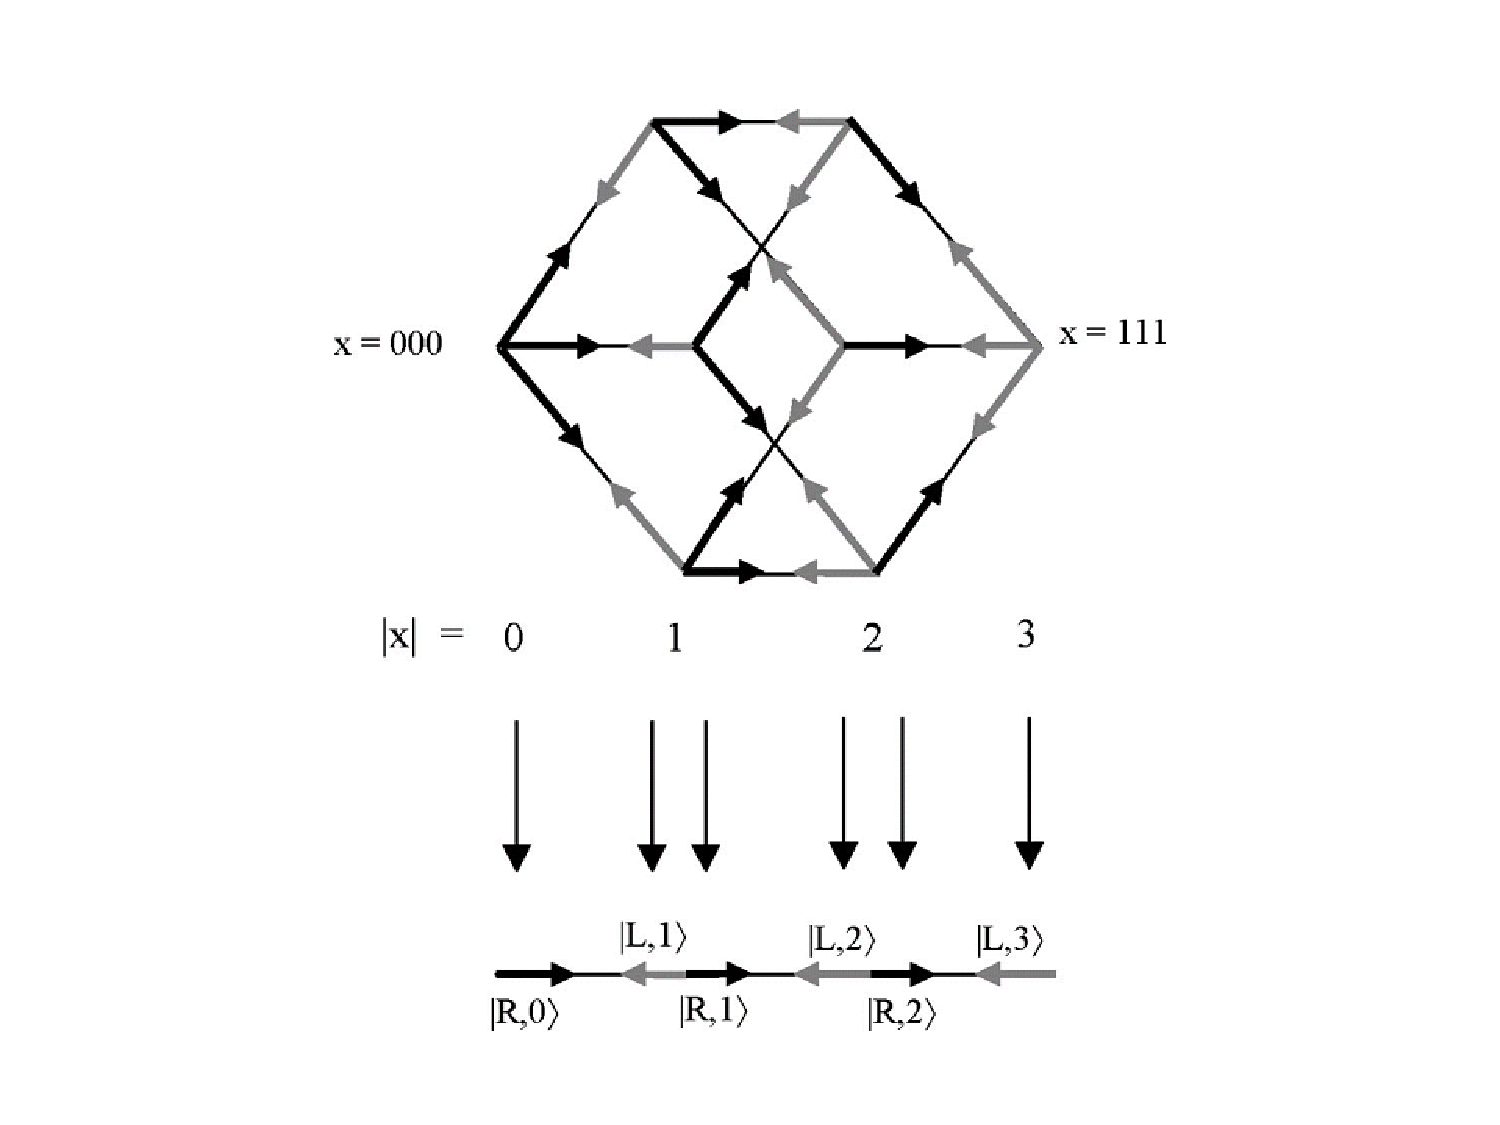
\includegraphics[width= 0.8\columnwidth]{figures/skw.pdf}
              \caption{SKW算法中的重要简化,把超立方体上的随机行走问题塌缩为了线上的随机行走问题。
              取自[Phys. Rev. A 67, 052307 (2003)]\cite{skw}。
              }
              \label{skw}
            \end{center}
 \end{figure}


\subsection{SKW算法与Grover算法的比较}

同为解决数据库搜索问题的量子搜索算法,SKW算法和Grover算法都有相同的加速效果。虽然本质上两个算法完全不同,但它们依然有很多相似的地方。

首先,两者的初态都是从所有二维矢量的等权重叠加态开始的,而且两者都用了Grover扩散算子$G$;两者都可以被看成是
二维子空间内的旋转;两者都利用了黑箱操作来给目标态标记上一个-1的相位;两者的时间复杂度都为$O(\sqrt{N})$;在两个算法中,都需要在特定的时间
进行测量以得到最大的成功概率。尽管如此,两个算法之间依然有很多重要的不同点,我们将介绍下两者的差异,并考虑这些差异如何影响算法的表现及执行的。

第一点不同是,Grover算法可以映射为由等权重叠加态$\left\vert \psi_{0} \right \rangle$与标记态$\left\vert 0 \right \rangle$张成的二维子空间内的旋转,算法中的每一次迭代都可以都可以对应到这个子空间内的旋转。SWK算法也可以看做是二维子空间内的
旋转,但和Grover算法相比有两点不同。其一,SKW算法只是近似地映射到二维子空间,不像Grover算法是精确的。其二,SWK算法中张成二维子空间的
矢量是$\left\vert \psi_{0} \right \rangle$和$\left\vert \psi_{1} \right \rangle$,而不是和精确的标记态$\left\vert 0 \right \rangle$。也就是说,SKW算法的末态并不是纯的标记态$\left\vert 0 \right \rangle$而是一个标记态和近邻态的线性组合,当然占主导地位的是标记态$\left\vert 0 \right \rangle$。因此,SKW算法包含一个对超立方体上的潜在拓扑结构的求迹过程。

另外一个重要的不同点是幺正操作的局域性。在SKW算法中,行走算子在超立方体的拓扑结构 上是局域的,也就是说行走只能发生在最近邻的$n$个点之间。硬币算子也只是在$n$维的硬币空间上变化。我们可以说SKW算法中的
幺正算子是$n$维局域的。在Grover算法中,映射算子则是高度非局域的。

再者,两个算法中的扩散算子$G$也是不同的。在Grover算法中,$G$被施加在整个$2^n$维搜索空间上,另一方面,SKW算法中的
扩散算子$G$则被用作量子硬币,只是作用于$n$维的硬币空间内。对于量子计算的物理实现来说,这点可能会很重要,因为对某些系统来说,实现
硬币空间内的算子要比实现Grover算法中要求的所有逻辑门要简单自然许多。最终决定哪个算法更有优势的还是物理实现的要求。

最后还有一个开放性的问题。两个算法在执行黑箱操作的时候也有一定的相似性。Grover算法中黑箱操作把目标态标记上相位-1,而SKW算法中则标上相位
$-\Gamma$ 在硬币上。这样做是因为此时的搜索结果非常容易分析,但目前并不确定这种标记是不是最优的或者唯一的。虽然数值分析的很多结果表明其他的一些标记方式也可以达到
搜索的目的,但相比于简单的$C_1 = -\Gamma$,对于复杂的硬币空间的分析也会非常的困难。在SKW算法中标记方式的选取目前仍然是一个开放问题。

关于SKW算法的一些发展及优化过程可以参见文献\cite{skw2,skw3,skw4,skw5},这些新的方案减少了SKW算法的复杂度并增加了搜索能力。

\section{SKW算法的实验实现}

“\emph{我做实验的唯一目的,就是给别的物理学家展示,量子理论究竟有多奇怪。}”

 \hspace{23em} \emph{--安顿·塞林格}

虽然已经有不少实验实现了包括离散型和连续型的量子随机行走过程\cite{rwexp1,rwexp2,rwexp3,rwexp4},但在我们的实验之前并没有
基于量子随机行走的算法的实验实现。在本节中,我们将介绍SKW算法的实验验证工作\cite{rw1},展示其超越经典算法的优越性。

\subsection{SKW算法的实验模型}

首先我们简单回顾一下原始的SKW算法。在搜索问题中,给定一个函数$\emph{f}\left(\emph{x}\right)$,当 $\emph{x}=\emph{a}$时 $\emph{f}\left(\emph{x}\right)=1$  , 否则 $\emph{f}\left(\emph{x}\right)=0$。我们的目标就是找到这个$\emph{a}$, 且 $0\leqslant \emph{a}\leqslant 2^n-1$。这种搜索问题就和在$n$维超立方体上的$\emph{N}=2^n$个节点中搜索一个标记的节点等价。

离散型随机行走可以简单地用幺正算子$U$的不断作用来描述。$U$被分为两个部分$U=SC$,其中$S$为行走算符,依据硬币空间的状态
进行行走操作,而$C$则类似于"抛硬币"操作,只不过这里抛的是量子硬币。为了搜索到标记的节点,SKW算法引入了一个由硬币算子决定的
黑箱操作:对要搜索的节点施加$C_1$,而对未标记的节点则施加$C_0$,并把这个新的硬币算子定义为$C'$。此时,整个新的幺正算子$U'$可以写成
$U'=SC'$,见图\ref{rwnet}。在把$U'$作用了
\begin{equation}
    t_{f}=\frac{\pi}{2}\sqrt{2^n}
\end{equation}
次后,我们可以通过测量得到标记态的概率为$\frac{1}{2}-O(n)$。

\begin{figure}[htbp]
            \begin{center}
              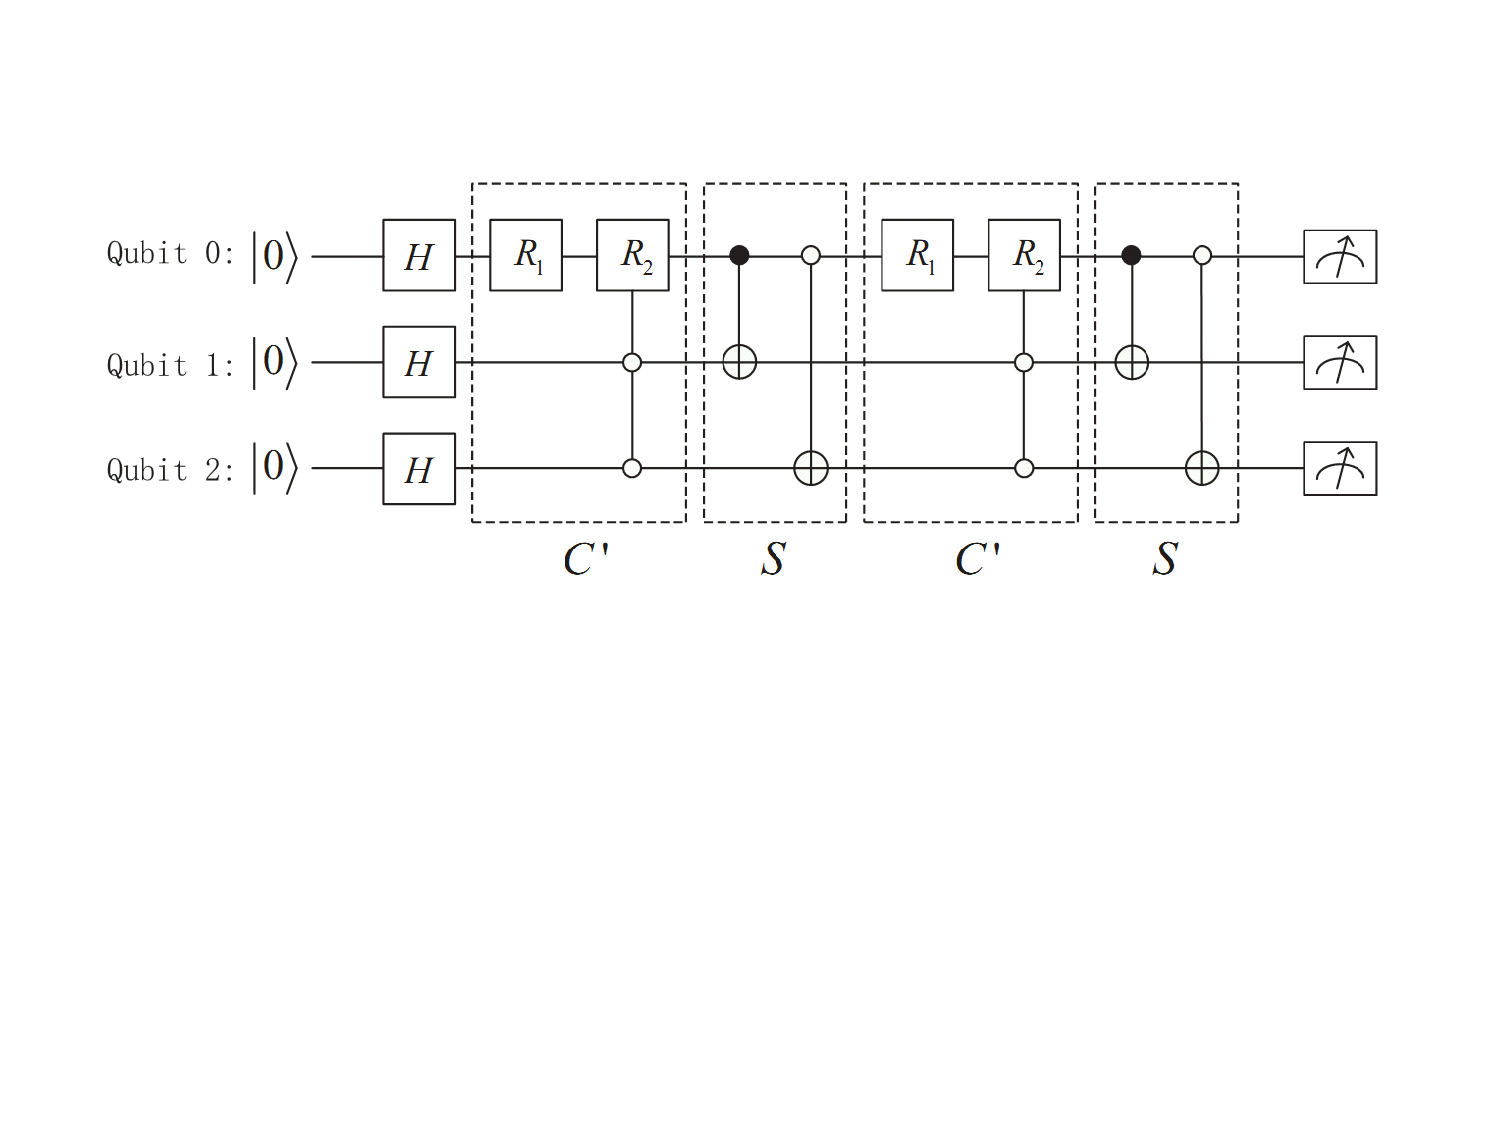
\includegraphics[width= 0.8\columnwidth]{figures/rwnet.pdf}
              \caption{实验中执行四选一搜索的网络图,目标态为$\left\vert 00
\right\rangle_{12}$。Qubit 0 被用作量子硬币,而qubit 1和qubit 2则是大的数据库。刚开始的Hadamard门为了产生所有计算基态的等权重叠加。实心点表示的是$\left\vert 1 \right\rangle$控制门,而空心点则是$\left\vert 0 \right\rangle$控制门。当数据库处于$\left\vert 00
\right\rangle_{12}$,即目标态的时候,执行$C_1=R_x^0(\pi/2)$(把qubit 0绕$\hat{x}$轴转$\pi/2$),否则的话执行$C_0=R_x^0(3\pi/2)$。在网络图中,我们用等价的效果$R_1=R_x^0(3\pi/2)$和
$R_2=R_x^0(-\pi)$替代。最后的测量则是要对所有的布居度进行重构,即测量末态密度矩阵的对角元。对于搜索其他的态,我们可以
得到类似的网络图。例如,目标态为$\left\vert 10
\right\rangle_{12}$时,我们只需要把三体相互作用的逻辑门的控制条件改为$\left\vert 10
\right\rangle_{12}$。  }\label{rwnet}
            \end{center}
 \end{figure}

当$n=2$时,我们需要3个qubit来验证SKW算法。第一个qubit被用作量子硬币,用qubit 0 标记。另外两个qubit被用作数据库存储,用qubit 1和qubit 2标记。我们的目标是从四个计算基矢${\left\vert 00 \right\rangle_{12},\left\vert 01
\right\rangle_{12},\left\vert 10 \right\rangle_{12},\left\vert 11
\right\rangle_{12}}$中找到$\left\vert \tau\sigma \right\rangle_{12} =
\left\vert \tau \right\rangle_{1}\otimes\left\vert \sigma
\right\rangle_{2} \left(\tau,\sigma=0,1 \right)$。这种四选一的算法网络图参见图\ref{rwnet}。假设我们的初态为$\left\vert 000 \right\rangle$。

(1)制备所有计算基矢的等权重叠加态
\begin{equation} \label{initial}
\left\vert \psi_{i} \right\rangle=\frac{\left\vert 0 \right\rangle_0+\left\vert 1 \right\rangle_0}{\sqrt{2}}\otimes\frac{\left\vert 0 \right\rangle_1+\left\vert 1 \right\rangle_1}{\sqrt{2}}\otimes\frac{\left\vert 0 \right\rangle_2+\left\vert 1 \right\rangle_2}{\sqrt{2}}.
\end{equation}
这一步可以通过在每个qubit上加一个Hadamard操作实现。

(2) 依据数据库的状态对硬币qubit进行幺正操作,即当数据库处于要搜索的态$\left\vert \tau\sigma \right\rangle_{12}$,并且
$C_0=R_x^0(3\pi/2)=e^{-i3\pi\sigma_x/4}$时,执行
\begin{equation}
C_1=R_x^0(\pi/2)=e^{-i\pi\sigma_x/4},
\end{equation}
否则的话执行
\begin{equation}
C_0=R_x^0(3\pi/2)=e^{-i3\pi\sigma_x/4}.
\end{equation}
我们可以利用图\ref{rwnet}中的形式进行简化,即等价地执行
\begin{equation}
R_1=R_x^0(3\pi/2)=e^{-i3\pi\sigma_x/4}
\end{equation}
和
\begin{equation}
R_2=R_x^0(-\pi)=e^{i\pi\sigma_x/2}
\end{equation}
操作。因此,整个硬币算子为
\begin{equation} \label{C'}
C'=C_0\otimes E_{12}+(C_1-C_0)\otimes\left\vert \tau\sigma
\right\rangle_{1212}\left\langle \tau\sigma \right\vert ,
\end{equation}
其中 $E_{12}$ 是数据上的单位矩阵。

在硬币算子后,数据库根据硬币qubit的状态执行行走操作$S$
\begin{eqnarray}
&&\left\vert 0 \right\rangle_{0}\left\vert 00 \right\rangle_{12}\Longleftrightarrow\left\vert 0 \right\rangle_{0}\left\vert 01 \right\rangle_{12}, \nonumber\\
&&\left\vert 0 \right\rangle_{0}\left\vert 10 \right\rangle_{12}\Longleftrightarrow\left\vert 0 \right\rangle_{0}\left\vert 11 \right\rangle_{12}, \nonumber\\
&&\left\vert 1 \right\rangle_{0}\left\vert 00 \right\rangle_{12}\Longleftrightarrow\left\vert 1 \right\rangle_{0}\left\vert 01 \right\rangle_{12}, \nonumber\\
&&\left\vert 1 \right\rangle_{0}\left\vert 01
\right\rangle_{12}\Longleftrightarrow\left\vert 1
\right\rangle_{0}\left\vert 11 \right\rangle_{12}.
\end{eqnarray}

(3) 将上面的行走重复两次得到末态
\begin{equation}
\left\vert \psi_{f} \right\rangle=\left( SC' \right)^2 \left\vert \psi_{i} \right\rangle.
\end{equation}

(4) 测量末态密度矩阵的所有对角元,以得到数据库qubit的布居度分布。例如,在目标态为${\left\vert 00 \right\rangle_{12}}$的情况,在把qubit 0求迹后,我们得到${\left\vert 00 \right\rangle_{12},\left\vert 01
\right\rangle_{12},\left\vert 10 \right\rangle_{12},\left\vert 11
\right\rangle_{12}}$的概率分别为0.5, 0.25, 0.25, 0。

当目标态为其他的状态时,我们可以通过改变控制条件得到类似的网络图及搜索过程。

\subsection{NMR实验实现}

我们的实验过程将分为三个部分来描述:实验系统,布居度测量方法及实验过程。

(a) \emph{实验系统}

\begin{figure}[htbp]
            \begin{center}
              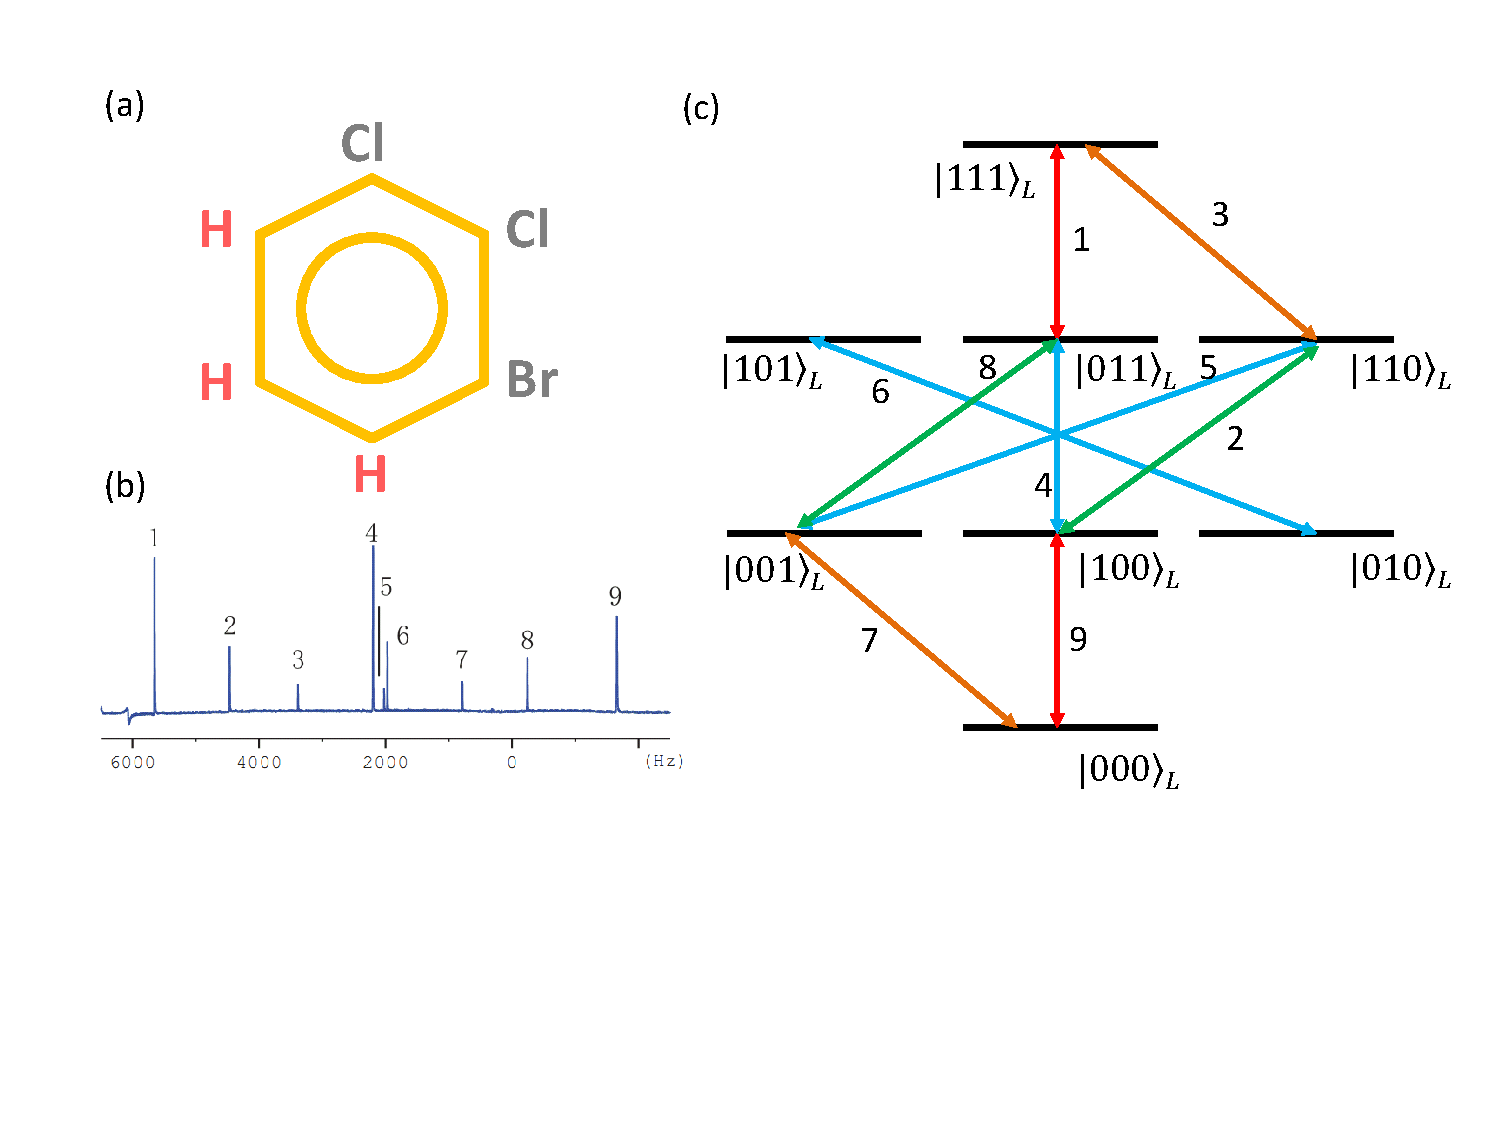
\includegraphics[width= 0.8\columnwidth]{figures/rwsample.pdf}
              \caption{(a) 1-Bromo-2,3-Dichlorobenzene的分子结构,三个$^1$H形成了一个3 qubit量子系统。(b) 热平衡态的NMR谱线。序号是根据可观测的跃迁频率的降序标记的。(c) 相应的本征能级之间的跃迁示意图。在$H_L$的表象中,1和9,2和8,3和7分别表征qubit 1, 2和3的跃迁。 }
              \label{rwsample}
            \end{center}
 \end{figure}

实验上我们采用的是3 qubit液晶NMR样品1-Bromo-2,3-Dichlorobenzene,溶剂是ZLI-1132。其分子结构见图\ref{rwsample}(a),三个$^1$H被用作三个qubit。实验是在Bruker
Avance 500-MHz的谱仪上完成的。样品的系统哈密顿量的形式为
\begin{eqnarray}\label{Hamiltonian}
\mathcal{H}=&&\sum\limits_{j=1}^3 {2\pi \nu _j } I_z^j  + \sum\limits_{j,k,j < k\leqslant 3} {2\pi} J_{jk} (I_x^j I_x^k  + I_y^j I_y^k+I_z^j I_z^k) \nonumber\\
&&+ \sum\limits_{j,k,j < k\leqslant 3} {2\pi} D_{jk} \left( {2I_z^j I_z^k  - I_x^j I_x^k  - I_y^j I_y^k } \right),
\end{eqnarray}
其中 $\nu_j$为第$j$个核自旋的化学位移,$\emph{D}_{jk}$和 $\emph{J}_{jk}$则分别是偶极耦合强度和标量耦合强度。在本实验中,$J$耦合是当作弱耦合近似处理的。由于哈密顿量中存在非对角元,
其本征态不再是简单的Zeeman直积态,而是它们的线性组合。虽然本征基矢也不再是计算基矢,我们依然利用计算基矢来储存和读取信息,但利用本征基矢来
读取NMR的谱线,因为在本征基矢中NMR的谱线更加易于理解。

\begin{figure}[htbp]
            \begin{center}
              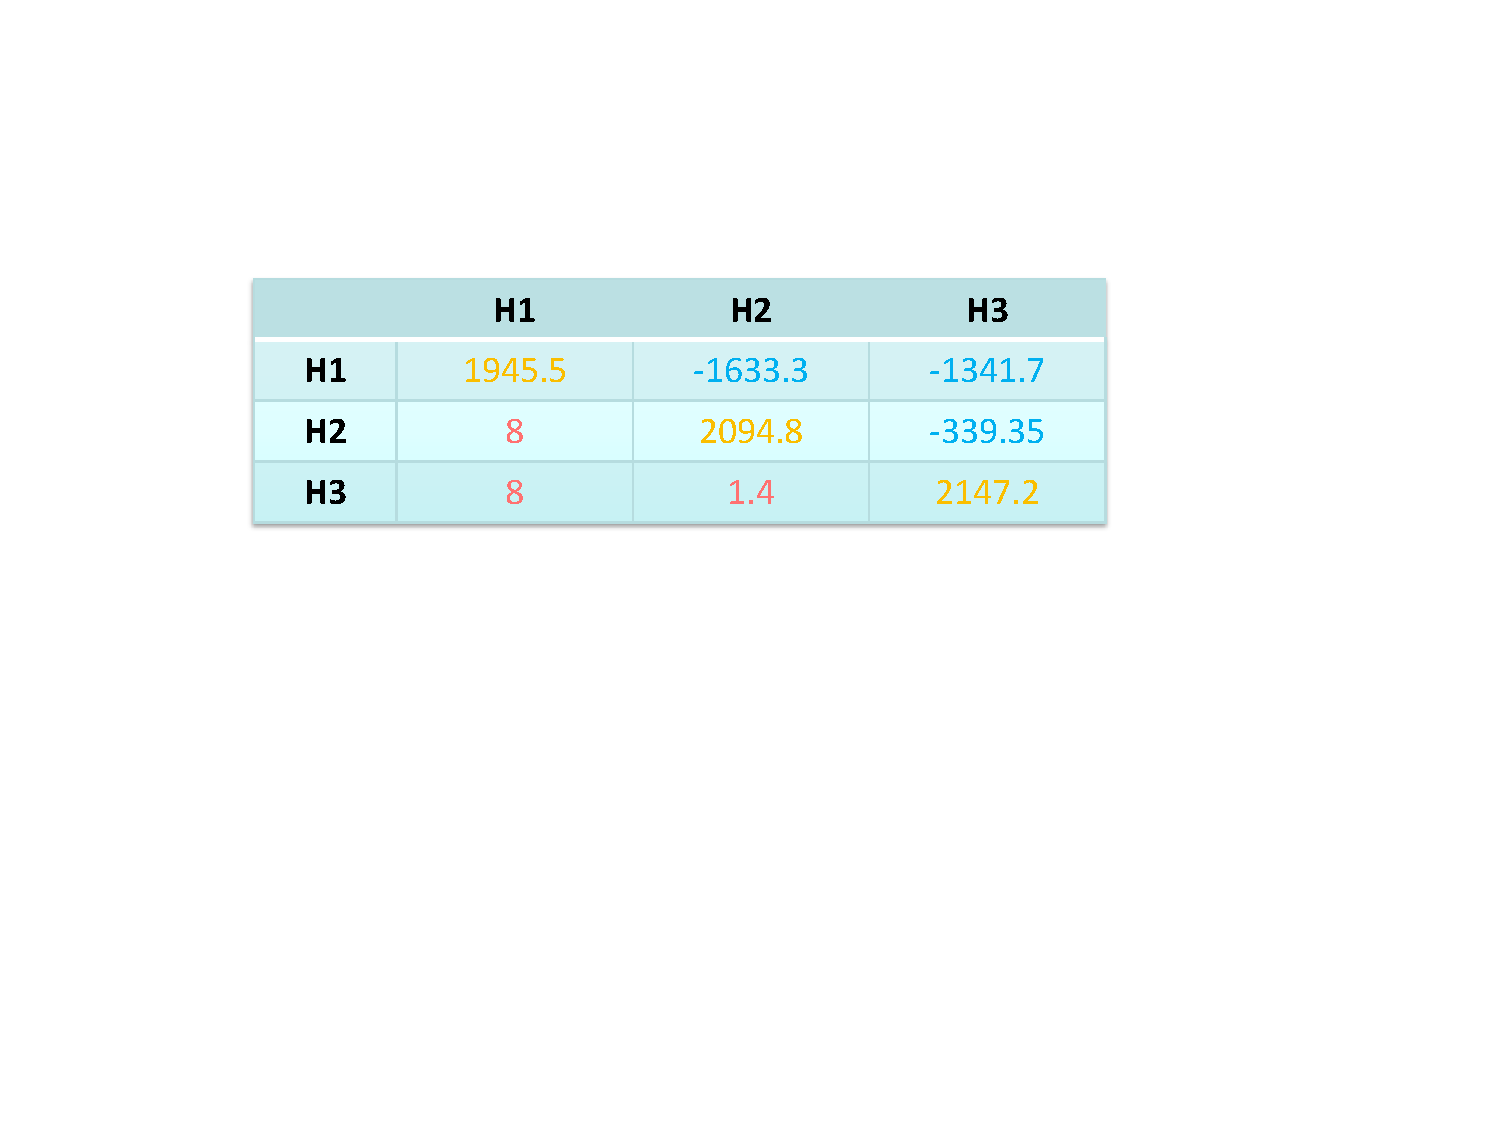
\includegraphics[width= 0.8\columnwidth]{figures/rwpara.pdf}
              \caption{ 1-Bromo-2,3-Dichlorobenzene的哈密顿量参数。这些参数是通过拟合谱线得到的,对角元(黄色)是化学位移,右上非对角元(蓝色)为偶极耦合的强度,左下非对角元(粉色)为$J$耦合的强度。
本表中所有的数值单位均为Hertz。}
              \label{rwpara}
            \end{center}
 \end{figure}

对系统的热平衡态$\rho_{th}=\sum\limits_{i=1}^3 \sigma_z^i$施加一个$\pi/2$脉冲后,我们可以得到该样品的热平衡态谱线(图\ref{rwsample}(b))。考虑分子的几何性质
并利用初始猜测的参数,我们可以不断拟合哈密顿量并和实验谱图对应,知道得到所有的参数大小。拟合得到的
结果见表\ref{rwpara}。在实验中,H$_2$被用作硬币qubit 0,而H$_1$和H$_3$则被用作数据库qubit 1和 qubit 2。

一旦确定了系统的哈密顿量,我们可以很容易地计算出其本征态$\left\vert \phi_{i} \right\rangle$($1\leqslant i\leqslant 8$)和本征值$E_i$。任意两个本征态$\left\vert \phi_{i} \right\rangle$ 和$\left\vert \phi_{j} \right\rangle$之间的相对跃迁强度$I_{ij}$可以通过
\begin{equation}
I_{ij}\varpropto \langle \phi_{i} | I^{+} | \phi_{j} \rangle ^2
\end{equation}
来计算,其中$I^+ = \sum_{k=1}^3 (I_x^k+iI_y^k)$。相应的跃迁频率为
\begin{equation} \label{transitions}
\omega_{ij}= E_i-E_j.
\end{equation}
经过计算,我们得到该系统中有15条可能的跃迁,其中6条的大小相对于1号跃迁来说小于$1\%$,因此在热平衡谱上
已经湮没在噪声之中。正是因为信噪比的原因,在图\ref{rwsample}(b)中我们只标记了9条主要的跃迁。

(b) \emph{布居度测量}

当哈密顿量确定后,我们考虑如何对其进行对角化。对于3 qubit的哈密顿量形式,要寻找一个对角化的幺正矩阵$U$并不困难。 对角化过程为
\begin{equation} \label{diag}
H_L = UH_SU^{\dag},
\end{equation}
其中$H_S$是系统的哈密顿量,而$H_L$是对角化的哈密顿量,或者可以看做是本征基矢下的哈密顿量。
对于系统哈密顿量来说,这种对角化过程并不是唯一的,实验上我们选择$U$为
\begin{eqnarray}\label{Transformation}
\left( {\begin{array}{*{20}c}
   {1} & {0} & {0} & {0} & {0} & {0} & {0} & {0}  \\
   {0} & {0.801} & {0.512} & {0} & {-0.303} & {0} & {0} & {0}  \\
   {0} & {0.375} & {-0.823} & {0} & {-0.420} & {0} & {0} & {0}  \\
   {0} & {0} & {0} & {0.810} & {0} & {0.126} & {0.559} & {0}  \\
   {0} & {-0.467} & {0.223} & {0} & {-0.856} & {0} & {0} & {0}  \\
   {0} & {0} & {0} & {0.458} & {0} & {-0.730} & {-0.508} & {0}  \\
   {0} & {0} & {0} & {0.344} & {0} & {0.672} & {-0.656} & {0}  \\
   {0} & {0} & {0} & {0} & {0} & {0} & {0} & {1}  \\ \nonumber
\end{array}} \right).
\end{eqnarray}
如此标记之后,所有的跃迁可以认为是两个本征态之间的跃迁了,且$\left\vert 000
\right\rangle_L=\left\vert 000 \right\rangle_S,\left\vert 111
\right\rangle_L=\left\vert 111 \right\rangle_S$,下标$L$和$S$分别表示本征基矢和计算基矢。所有的9个可观测的跃迁现在都可以被标记在
本征态的跃迁示意图中(图\ref{rwsample}(c))。

\begin{figure}[htbp]
            \begin{center}
              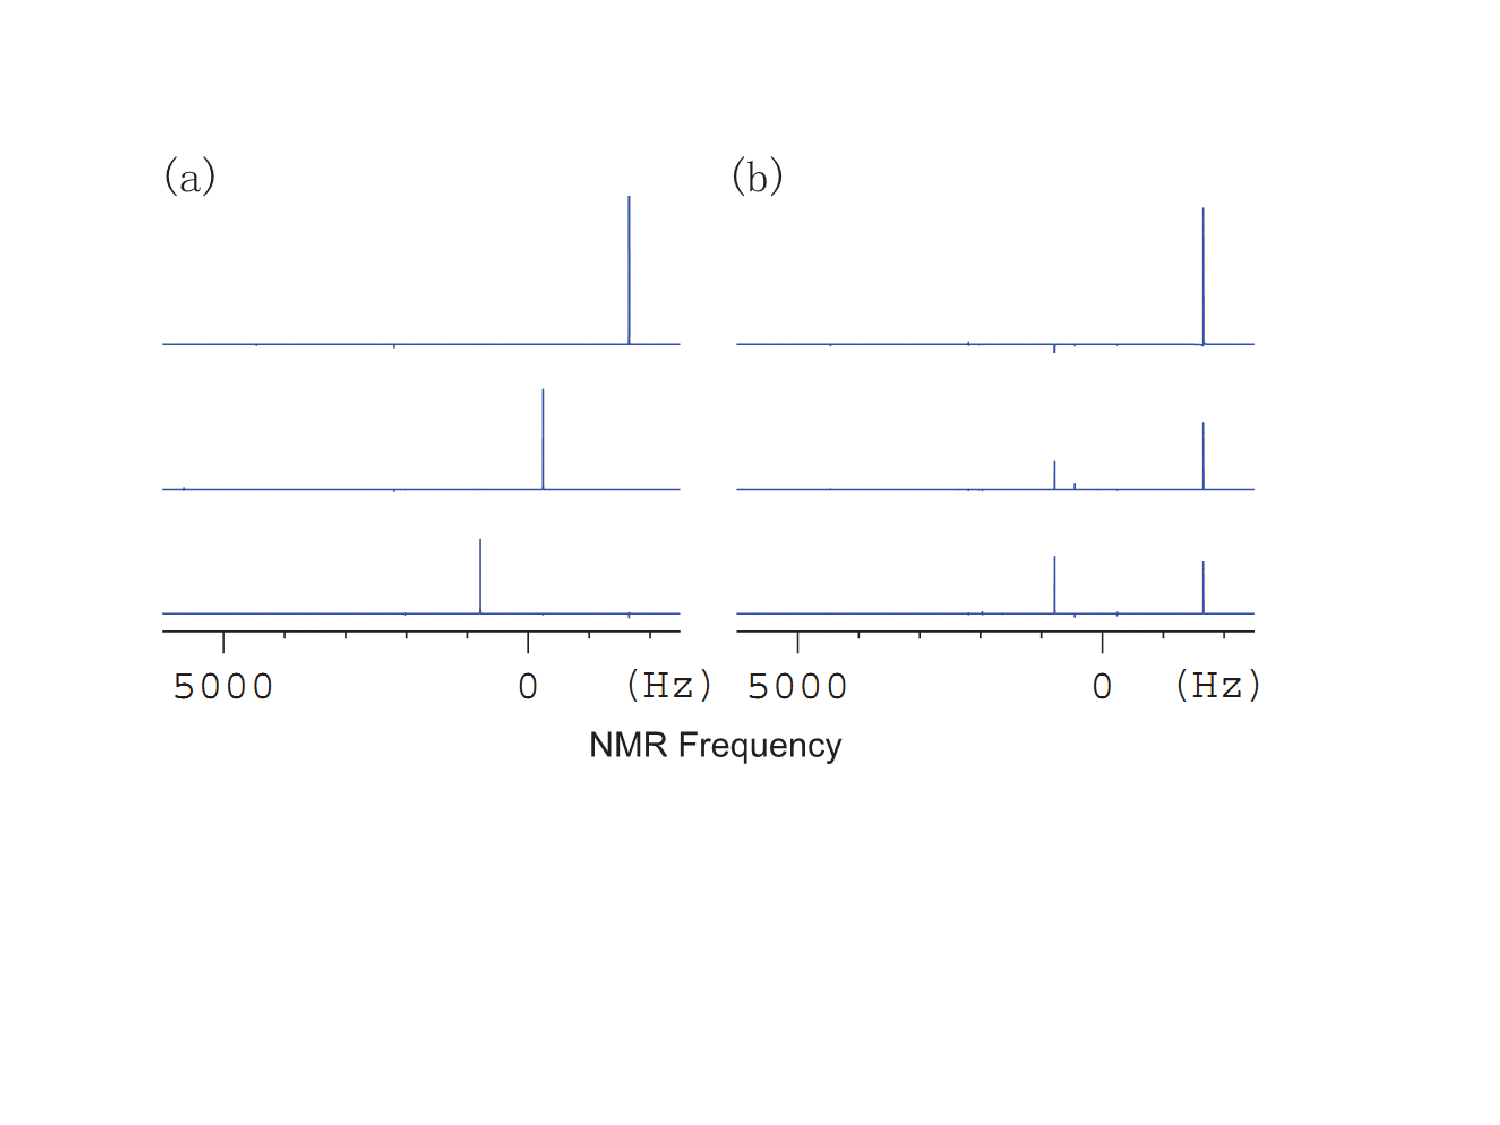
\includegraphics[width= 0.8\columnwidth]{figures/rwpps.pdf}
              \caption{PPS的观测模拟结果。(a) 观测脉冲为$UR_1^y(\pi/2),UR_2^y(\pi/2)R_3^y(\pi),UR_3^y(\pi/2)$时的观测结果。(b) 传统的观测脉冲$R_1^y(\pi/2),R_2^y(\pi/2),R_3^y(\pi/2)$得到的谱线。我们可以看到(a)中的谱线比(b)容易理解很多。}
              \label{rwpps}
            \end{center}
 \end{figure}

不失一般性,我们关注最右边的三条跃迁7,8 和9。考虑初态$\rho_S$为纯态$(\left\vert 000 \right\rangle\left\langle 000
\right\vert)_S$的简单情况,在弱耦合的液体NMR中,如果我们用一个$R_y^1(\pi/2)$脉冲激发qubit 1,我们可以在谱线上观测到一条峰,这也是液体NMR中观测PPS的通用方法。但是,在液晶NMR中,单个qubit的旋转并不会
形成一条单峰,而是一些相关峰的组合(图\ref{rwpps}(b))。可以看出这么复杂的谱线分布并不适合读出密度矩阵的信息,而解决这个问题的直观想法是利用本征基矢。
我们尝试在序列中的读出脉冲后再加上对角化矩阵$U$,并观察此时的读出结果。图\ref{rwpps}(a)给出了对纯态$(\left\vert 000 \right\rangle\left\langle 000 \right\vert)_S$ 施加三个读出脉冲
$UR_1^y(\pi/2),UR_2^y(\pi/2)R_3^y(\pi),UR_3^y(\pi/2)$后的NMR谱线。第二个脉冲利用了$R_3^y(\pi)$的旋转是因为8号跃迁是
$\left\vert 001 \right\rangle_L\rightarrow \left\vert 011
\right\rangle_L$,而非$\left\vert 000 \right\rangle_L\rightarrow
\left\vert 010 \right\rangle_L$。从模拟的结果看,NMR谱线展示了非常好的结果,和液体NMR非常类似。

为了读出任意密度矩阵$\rho_S$的对角元,我们也可以利用上面提到的方法。不妨把所有的布居度$(\left\vert 000 \right\rangle\left\langle 000
\right\vert)_S$ 到$(\left\vert 111 \right\rangle\left\langle 111
\right\vert)_S$ 分别定义为$P(1)$到$P(8)$,而$UR_1^y(\pi/2)$激发的跃迁为9号跃迁$\left\vert 000 \right\rangle_L\rightarrow \left\vert
100 \right\rangle_L$ 及$\left\vert 100 \right\rangle_L\rightarrow
\left\vert 000 \right\rangle_L$。通过这条谱线,我们就可以得到$P(1)-P(5)$的值。表\ref{rwread}给出了所有的通过读出脉冲可以得到的$P(i)-P(j)$
的值。结合归一化条件$\sum_{i=1}^8P(i)=1$,我们可以求解所有的布居度的值。

\begin{figure}[htbp]
            \begin{center}
              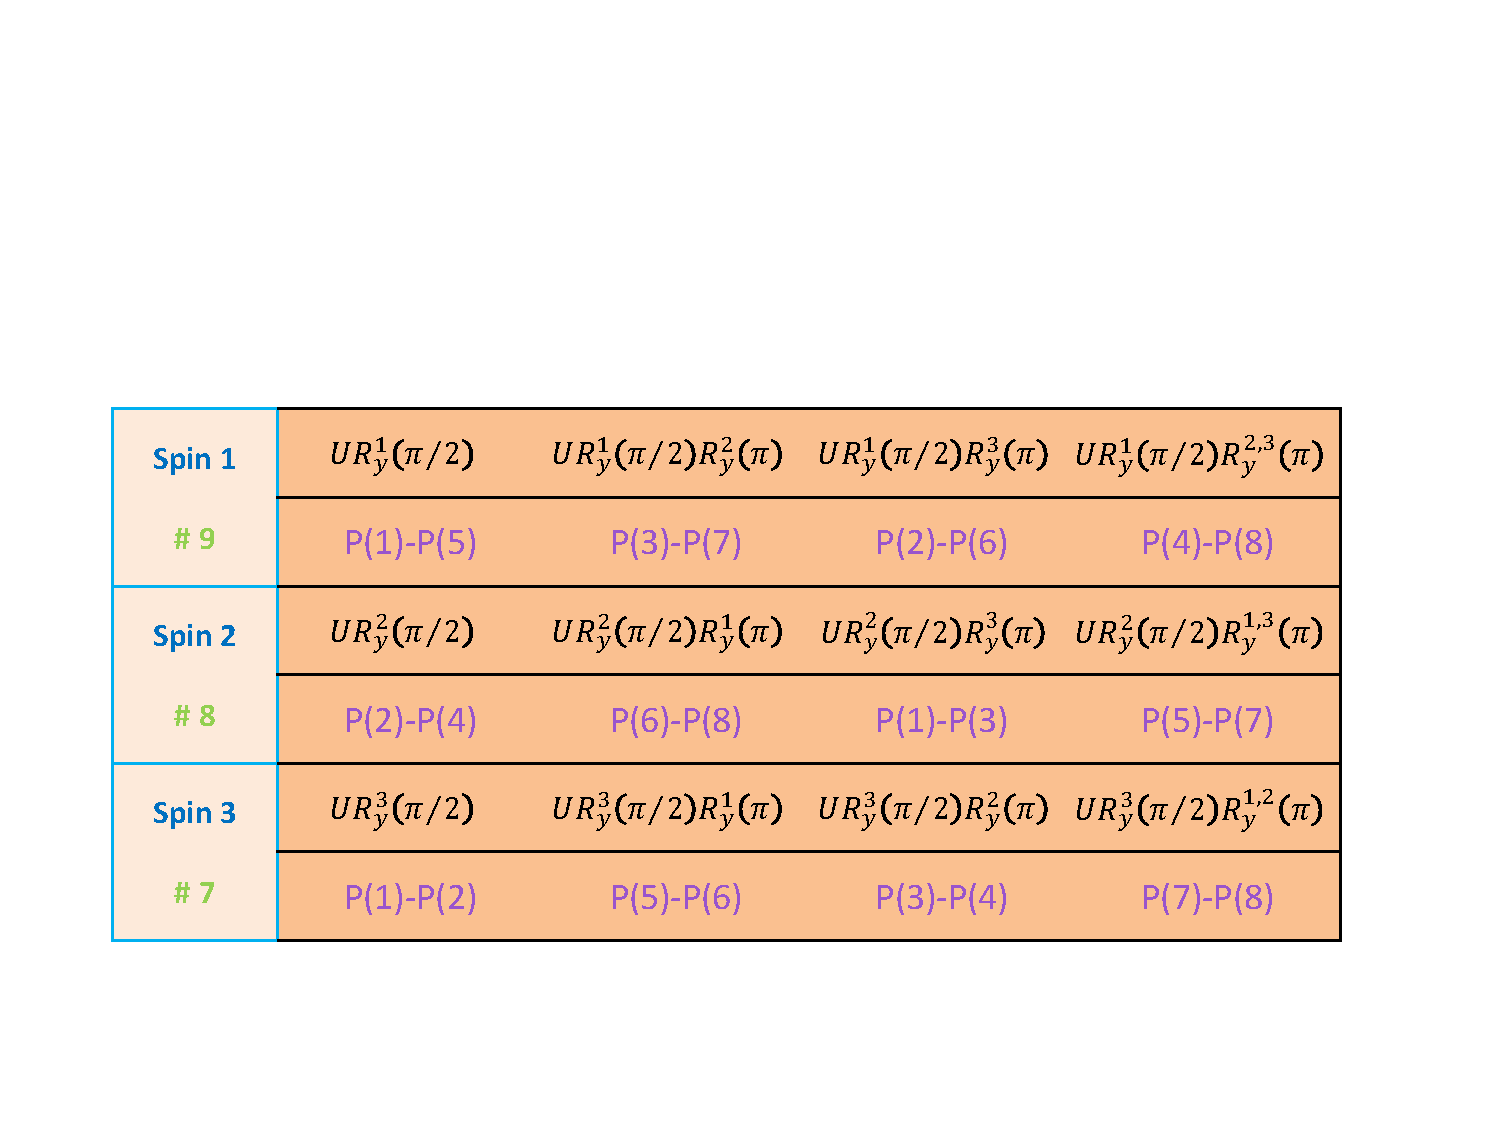
\includegraphics[width= 0.8\columnwidth]{figures/rwread.pdf}
              \caption{读出脉冲以及相关的布居度之差$P(i)-P(j)$。实验结果都是在9号,8号及7号跃迁上观测的。结合归一化条件$\sum_{i=1}^8P(i)=1$,所有的
对角元都可以求解出来。}
              \label{rwread}
            \end{center}
 \end{figure}

(c) \emph{实验过程}

整个实验过程被分为三步:PPS制备,量子随机行走搜索过程以及布居度测量。从热平衡态出发,我们首先
要制备PPS
\begin{equation}
\rho_{000}=\frac{1-\epsilon
}{8}\mathbf{1}+\epsilon \left\vert 000 \right\rangle \left\langle
000\right\vert,
\end{equation}
其中$\mathbf{1}$是单位阵,而$\epsilon$是系统的极化度。我们利用了GRAPE脉冲及梯度场实现了PPS制备,数值模拟的保真度为
0.977。在本征基矢中观测PPS的结果参见图\ref{rwspec}(a)。可以看出在忽略一些小的误差后,这就是一条纯粹的吸收峰。

\begin{figure}[htbp]
            \begin{center}
              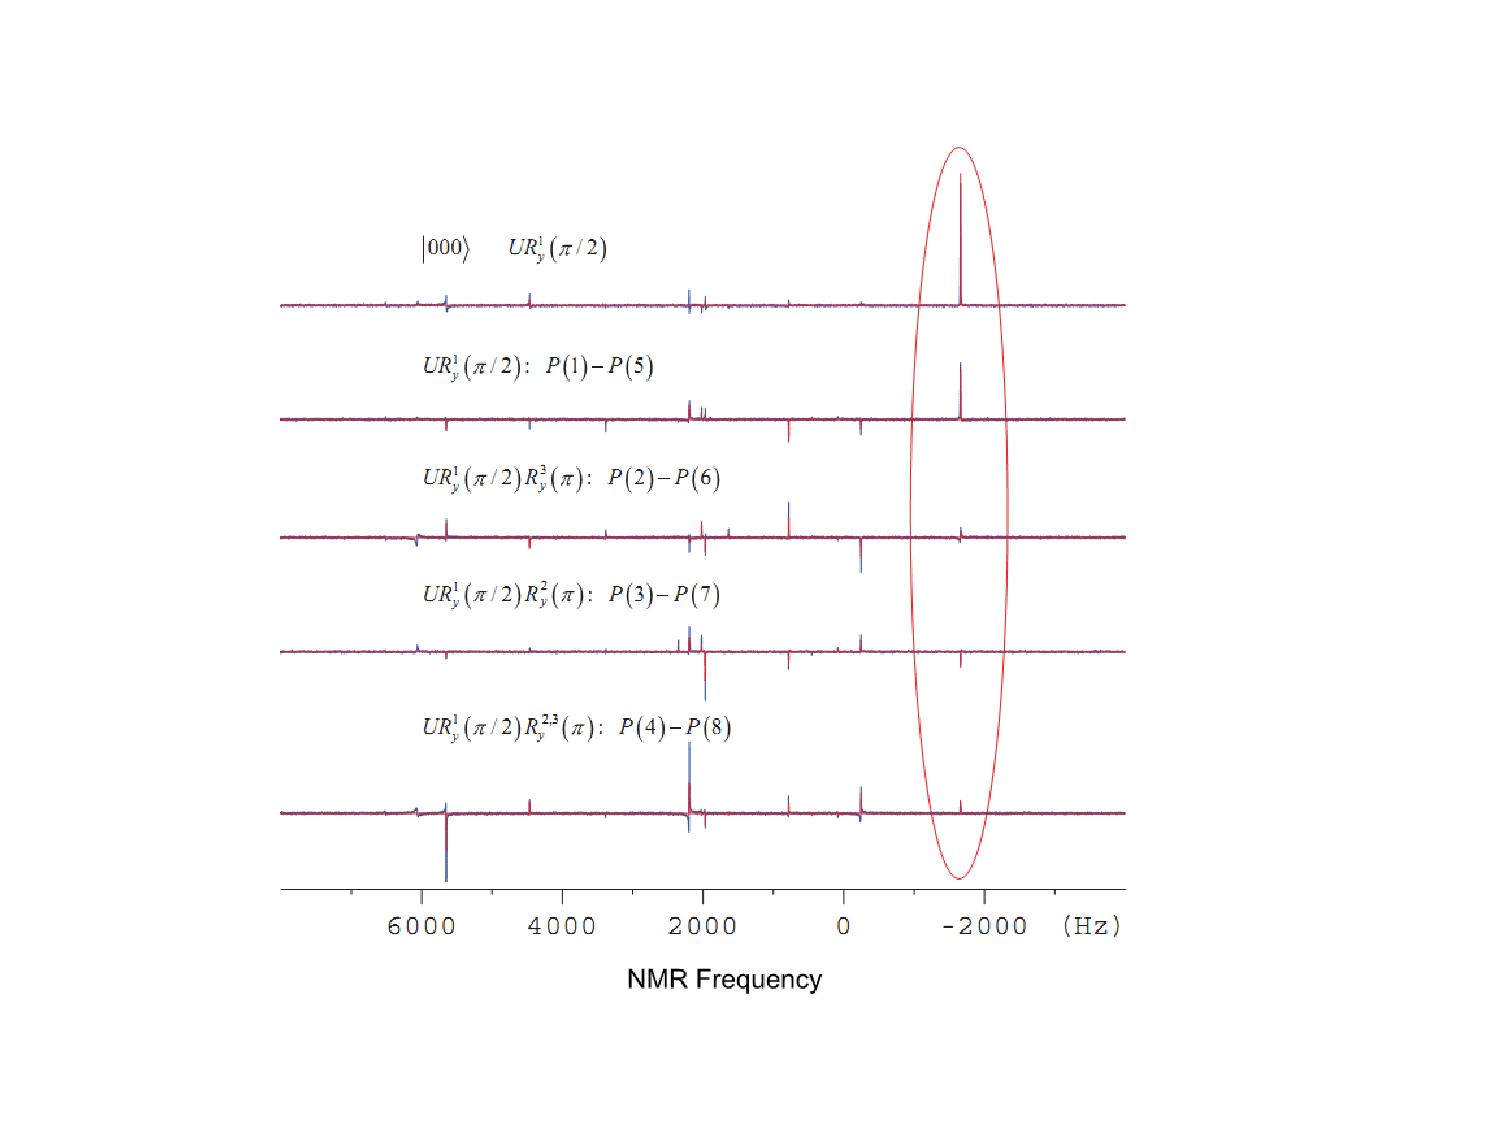
\includegraphics[width= 0.8\columnwidth]{figures/rwspec.pdf}
              \caption{测量自旋1的对角元的NMR谱线。蓝色和红色的谱线分别为实验和模拟结果。我们仅仅关注9号跃迁(椭圆内的峰)来读出
$P(1)-P(5)$,$P(2)-P(6)$,$P(3)-P(7)$ 和 $P(4)-P(8)$,利用的是图上标记的四个读出算子。第一个谱图是PPS$\left\vert
000 \right\rangle$的观测结果,被用作后面积分的基准。四个布居度之差的理论结果为0.375,0, -0.125,0.125,而实验结果为0.383,0.050,-0.061和 0.093。}
              \label{rwspec}
            \end{center}
 \end{figure}

量子随机行走搜索过程则包含两个部分:初态$|+\rangle^{\otimes3}$
($|+\rangle=(|0\rangle+|1\rangle)/\sqrt{2}$)的制备和两次迭代的幺正演化。我们把这两个过程利用GRAPE打包到了一起,
形成了一个20ms分为250小片的GRAPE脉冲,其保真度高于0.990。表\ref{rwread}中的所有读出算子也有20ms且保真度高于0.990的脉冲进行了
打包。9号跃迁上的观测结果见图\ref{rwspec}(a),最后我们得到的末态密度矩阵的对角元与理论值相比,其保真度为0.983,而搜索到
$\left\vert 00
\right\rangle$, $\left\vert 01 \right\rangle$, $\left\vert
10 \right\rangle$, $\left\vert 11 \right\rangle$的概率分别为0.513, 0.232,0.197, 0.058。至此就证明我们完成了基于SKW算法的$\left\vert 00 \right\rangle$的搜索。

除了$\left\vert 00 \right\rangle$之外,我们还把目标态改为了$\left\vert 01 \right\rangle$, $\left\vert 10
\right\rangle$ 和 $\left\vert 11 \right\rangle$。执行SKW算法后的实验结果绘制在图\ref{rwresult}上。可以看出实验和理论结果是一致的,
而它们之间微小的误差主要来源于退相干,射频场的不均匀性及GRAPE的不完美性。为了衡量实验结果,我们在图\ref{rwspec}中还给出了利用Topspin
软件中NMR-sim软件的模拟结果。在给出了哈密顿量,GRAPE脉冲与脉冲序列后,该软件可以不引入实验不完美性给出模拟谱线。模拟谱和实验谱在
线宽上的微小差别来源于模拟过程中的$T_2$和实验有略微的区别。在可接受的误差范围内,模拟和实验的线宽是一致的。


\begin{figure}[htbp]
            \begin{center}
              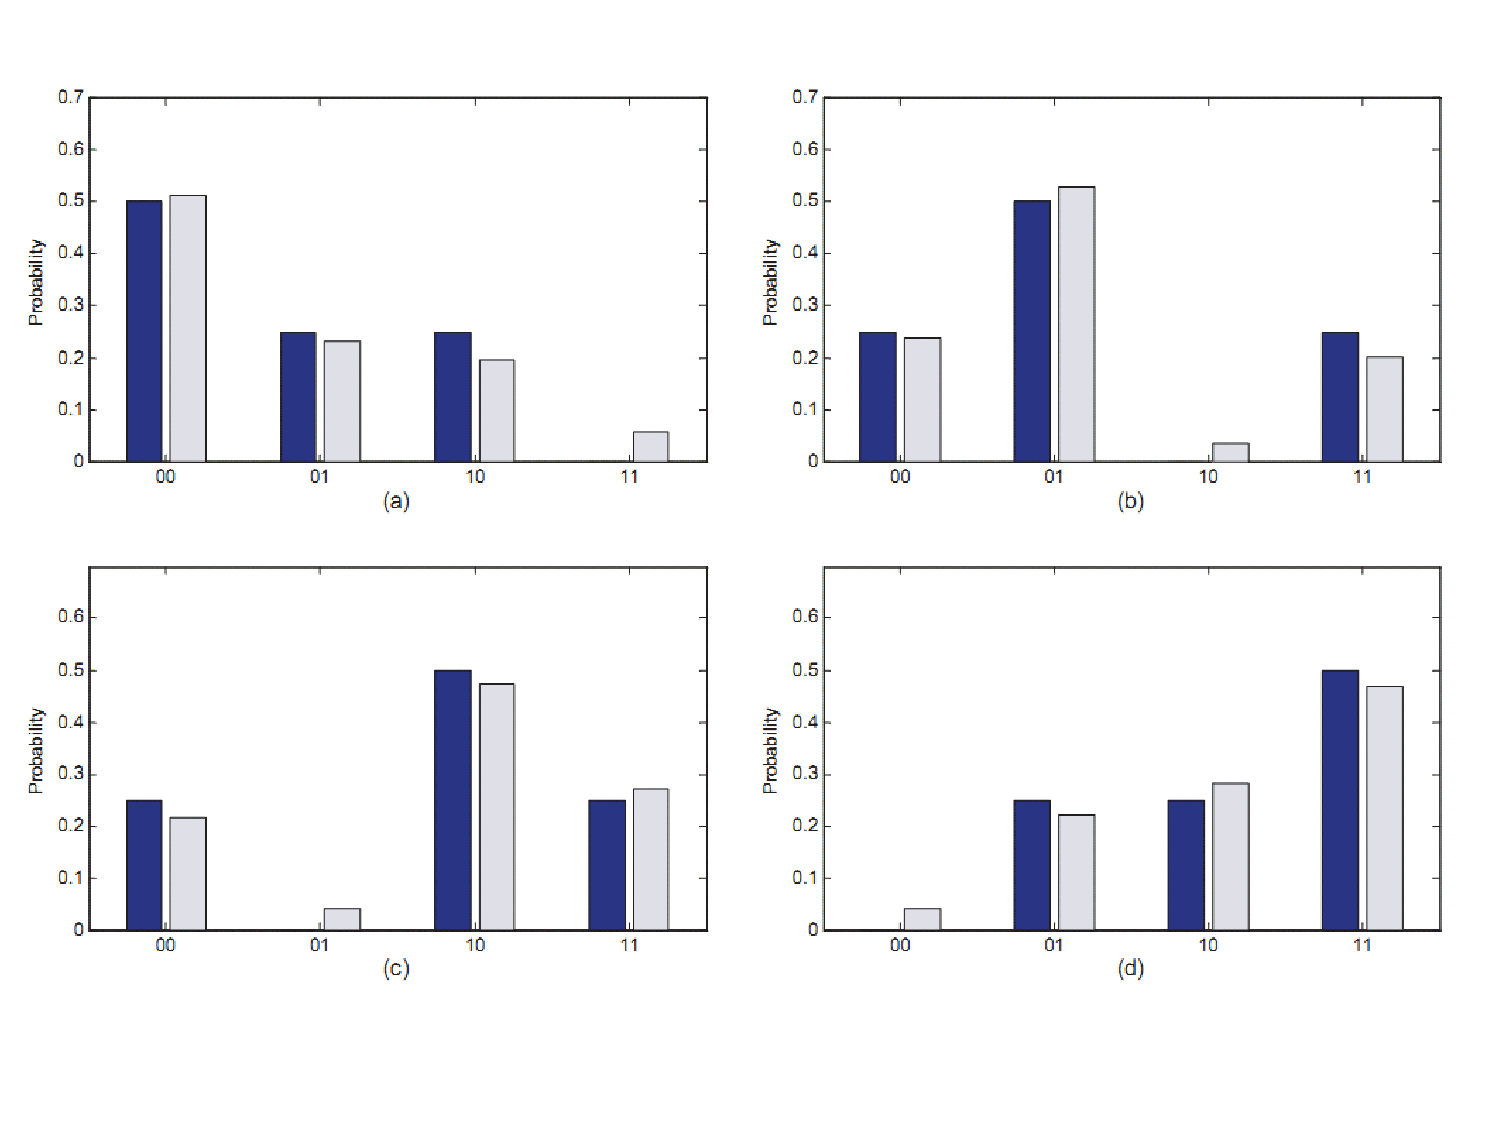
\includegraphics[width= 0.8\columnwidth]{figures/rwresult.pdf}
              \caption{SKW算法的实验结果。(a), (b), (c), (d) 分别对应于搜索$\left\vert 00 \right\rangle_{12}$, $\left\vert 01
\right\rangle_{12}$,$\left\vert 10 \right\rangle_{12}$ 和
$\left\vert 11 \right\rangle_{12}$的情况。蓝条代表的是理论预期,而灰条则是实验结果。}
              \label{rwresult}
            \end{center}
 \end{figure}

\subsection{实验总结及讨论}

我们在实验上验证了四选一情况的SKW算法。该算法可以通过$\emph{O}(\sqrt{\emph{N}})$次黑箱操作,来实现包含$N$个
元素的数据库的搜索,并得到和Grover算法类似的加速能力。实验是在3 qubit强耦合的液晶NMR体系上完成的,而GRAPE脉冲的利用以很高的保真度实现了幺正操作和对角元的测量。
从实验结果来看,它们和理论预期符合的很好,也展示了SKW算法的优越性。

本实验中发展的这套针对液晶NMR体系量子计算的方法可以扩展到更多qubit的系统上。在引入更多qubit后,主要的挑战来源于
GRAPE脉冲的计算和哈密顿量对角化的困难。当然,随着算法的改进,这些困难在未来都可能被克服,而且这套方法在低量子位上也已被证明
是非常适合及有效的。

本节的工作已发表在Phys. Rev. A 81, 022308 (2010)\cite{rw1}上。 